% COMS 6998 midterm presentation, 6 Nov 2026. 5 min + 1 min Q&A, 5-6 slides.
% Brief (Zishen, 1 Nov): intro slide, research problem, approach, progress
% and findings, next steps.
% Sources: Pulak's Nov 5 Google Slides text (Research/5thNov-Updates.txt),
% the kickoff deck (1-kickoff), the experiment plan (2-experiments), the final
% Nov 5 deck (slides/slides-5nov/final), notes/usecases-notes/preliminary-answers.md.
% Lines marked % CLAUDE were written or combined by Claude: rewrite them.
\documentclass[11pt,aspectratio=169]{beamer}
\usepackage{amsmath,amssymb,booktabs,graphicx,xcolor,tikz}
\usetikzlibrary{arrows.meta,positioning,calc,decorations.pathreplacing}

\definecolor{accent}{HTML}{2E75B6}
\definecolor{red2}{HTML}{C0392B}
\definecolor{green2}{HTML}{27AE60}
\definecolor{orange2}{HTML}{E67E22}
\definecolor{gray2}{HTML}{7F8C8D}
\definecolor{purple2}{HTML}{8E44AD}
\definecolor{cpuc}{HTML}{F6E9C6}
\definecolor{cpud}{HTML}{9A7420}
\definecolor{gpuc}{HTML}{D6E2EE}
\definecolor{gpud}{HTML}{3F6286}

\setbeamertemplate{navigation symbols}{}
\setbeamersize{text margin left=1.0cm,text margin right=1.0cm}
\setbeamercolor{normal text}{fg=black,bg=white}
\setbeamercolor{frametitle}{fg=black,bg=white}
\setbeamercolor{structure}{fg=black}
\setbeamercolor{block title}{fg=black,bg=black!10}
\setbeamercolor{block body}{fg=black,bg=black!3}
\setbeamerfont{title}{size=\large,series=\bfseries}
\setbeamerfont{frametitle}{size=\normalsize,series=\bfseries}
\setbeamerfont{block title}{size=\small,series=\bfseries}
\setbeamertemplate{footline}{\leavevmode\hbox{\begin{beamercolorbox}[wd=\paperwidth,ht=2.5ex,dp=1ex,rightskip=0.9cm]{author in head/foot}\hfill\insertframenumber\end{beamercolorbox}}}

\tikzset{
  wb/.style={draw, fill=white, rounded corners=2pt, line width=1.1pt, align=center, inner sep=4pt},
  arr/.style={-{Stealth[length=5pt]}, line width=0.8pt},
  lbl/.style={font=\scriptsize, text=black!70, align=center},
  tsn/.style={circle, fill=black, text=white, font=\tiny\bfseries, inner sep=0pt, minimum size=3.4mm},
}
\newcommand{\ts}[1]{\tikz[baseline=(c.base)]\node[circle,fill=black,text=white,font=\tiny\bfseries,inner sep=0pt,minimum size=3.2mm](c){#1};}
\setlength{\parindent}{0pt}
\newcommand{\todo}[1]{\textcolor{red2}{[#1]}}

\begin{document}

% ==================================================================
% 1. You (first 30 seconds)
\begin{frame}[plain]
\vspace{1.2cm}
{\large\bfseries Latency-Bound Inference on GPUs}\\[0.3em]
{\small My Master's thesis}

\vspace{1.2cm}
{\bfseries Pulak Mehrotra}\\[0.6em]
\small
Background in Wireless Systems and GPU Systems
\\[0.6em]
Currently interested in ML systems: making single-GPU inference stable and predictable. % CLAUDE

\vfill
{\scriptsize\color{gray2} COMS 6998, midterm presentation, 6 November 2026}
\end{frame}

% ==================================================================
% 2. Research problem
\begin{frame}{Do inference frameworks miss their deadlines in a loop, and why?} % CLAUDE (joins kickoff Q1 and Q2)

\vspace{0.05cm}
\begin{center}
\resizebox{0.62\linewidth}{!}{%
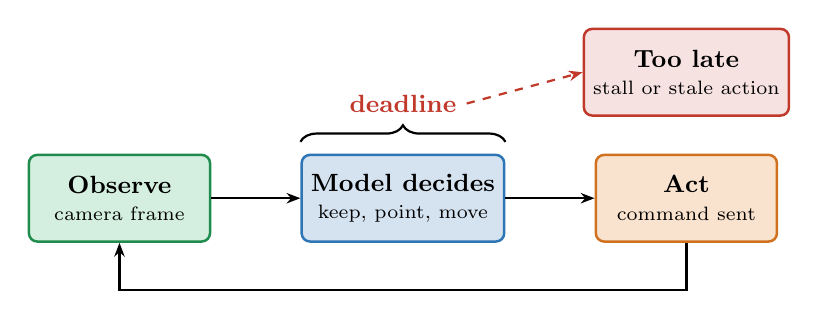
\begin{tikzpicture}[
  every node/.style={font=\small},
  box/.style={draw, rounded corners=3pt, minimum width=2.3cm, minimum height=1.1cm, align=center, line width=0.9pt},
]
  \node[box, fill=green2!20, draw=green2!80!black]   (obs) at (0,0)   {\textbf{Observe}\\[-1pt]{\scriptsize camera frame}};
  \node[box, fill=accent!20, draw=accent]            (dec) at (3.6,0) {\textbf{Model decides}\\[-1pt]{\scriptsize keep, point, move}};
  \node[box, fill=orange2!22, draw=orange2!90!black] (act) at (7.2,0) {\textbf{Act}\\[-1pt]{\scriptsize command sent}};
  \draw[arr] (obs) -- (dec);
  \draw[arr] (dec) -- (act);
  \draw[arr] (act.south) -- ++(0,-0.6) -| (obs.south);
  \draw[decorate, decoration={brace, amplitude=6pt}, line width=0.8pt]
    ($(dec.north west)+(0,0.15)$) -- ($(dec.north east)+(0,0.15)$)
    node[midway, above=7pt, font=\small\bfseries, text=red2] (dl) {deadline};
  \node[box, fill=red2!14, draw=red2, minimum width=2.6cm] (miss) at (7.2,1.6)
    {\textbf{Too late}\\[-1pt]{\scriptsize stall or stale action}};
  \draw[arr, red2, dashed] (dl.east) -- (miss.west);
\end{tikzpicture}}
\end{center}

\vspace{0.05cm}
% use cases: kickoff "Looped use cases" table; budgets from 2-experiments
\begin{center}
\footnotesize
\renewcommand{\arraystretch}{1.3}
\begin{tabular}{@{}l l l@{}}
\textcolor{accent}{\textbf{Space}}, VLM & keep or drop each image before the next one arrives & 1.5 s \\ % CLAUDE (combined)
\textcolor{orange2!90!black}{\textbf{Robot}}, VLA & send the next arm actions before the current ones run out & 100 to 250 ms \\ % CLAUDE (combined)
\end{tabular}
\end{center}

\vspace{0.15cm}
\small
Most work reduces interference or makes VLAs and VLMs run faster.\\[0.3em]
No work first nails down where the non-determinism in edge inference comes from and then tries to stabilise it.

\end{frame}

% ==================================================================
% 3. Approach: the setup
\begin{frame}{Measuring where the latency lies on real hardware}

\vspace{-0.1cm}
{\centering\small Each experiment is a model + the interference it has to deal with.\par}

\vspace{-0.05cm}
\begin{center}
\resizebox{0.8\linewidth}{!}{%
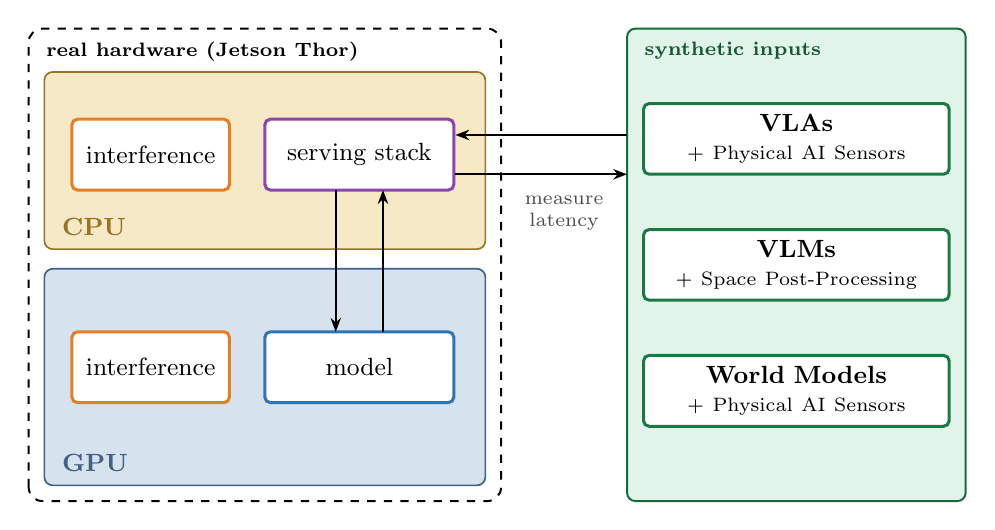
\begin{tikzpicture}[every node/.style={font=\small}]
  % ---- real hardware ----
  \draw[dashed, line width=0.7pt, rounded corners=5pt] (0,0) rectangle (6.0,6.0);
  \node[anchor=north west, font=\scriptsize\bfseries] at (0.1,5.95) {real hardware (Jetson Thor)};

  \draw[fill=cpuc, draw=cpud, line width=0.6pt, rounded corners=3pt] (0.2,3.2) rectangle (5.8,5.45);
  \node[anchor=south west, font=\small\bfseries, text=cpud] at (0.3,3.25) {CPU};
  \draw[fill=gpuc, draw=gpud, line width=0.6pt, rounded corners=3pt] (0.2,0.2) rectangle (5.8,2.95);
  \node[anchor=south west, font=\small\bfseries, text=gpud] at (0.3,0.25) {GPU};

  \node[wb, draw=purple2, minimum width=2.4cm, minimum height=0.9cm] (stk) at (4.2,4.4) {serving stack};
  \node[wb, draw=orange2, minimum width=2.0cm, minimum height=0.9cm] at (1.55,4.4) {interference};
  \node[wb, draw=accent, minimum width=2.4cm, minimum height=0.9cm] (mdl) at (4.2,1.7) {model};
  \node[wb, draw=orange2, minimum width=2.0cm, minimum height=0.9cm] at (1.55,1.7) {interference};

  \draw[arr] (3.9,3.95) -- (3.9,2.15);
  \draw[arr] (4.5,2.15) -- (4.5,3.95);

  % ---- synthetic inputs ----
  \draw[fill=green2!14, draw=green2!60!black, line width=0.7pt, rounded corners=3pt] (7.6,0) rectangle (11.9,6.0);
  \node[anchor=north west, font=\scriptsize\bfseries, text=green2!50!black] at (7.7,5.95) {synthetic inputs};
  \node[wb, draw=green2!70!black, text width=3.6cm] at (9.75,4.6) {\textbf{VLAs}\\[-1pt]{\scriptsize + Physical AI Sensors}};
  \node[wb, draw=green2!70!black, text width=3.6cm] at (9.75,3.0) {\textbf{VLMs}\\[-1pt]{\scriptsize + Space Post-Processing}};
  \node[wb, draw=green2!70!black, text width=3.6cm] at (9.75,1.4) {\textbf{World Models}\\[-1pt]{\scriptsize + Physical AI Sensors}};

  % ---- the loop ----
  \draw[arr] (7.6,4.65) -- (stk.east |- 0,4.65);
  \draw[arr] (stk.east |- 0,4.15) -- (7.6,4.15);
  \node[lbl, anchor=north] at (6.8,4.0) {measure\\latency};
\end{tikzpicture}}
\end{center}

\vspace{0.05cm}
{\centering\small We run the loop on real hardware, serving stacks and models with synthetic inputs,\\ and measure latency.\par}

\end{frame}

% ==================================================================
% 4. Approach: what one measurement is
\begin{frame}{The anatomy of a request in edge inference}

\vspace{0.2cm}
\begin{center}
\resizebox{0.9\linewidth}{!}{%
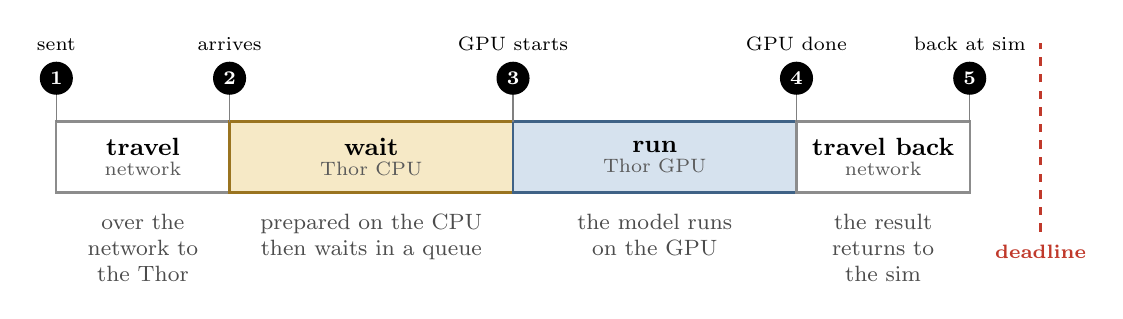
\begin{tikzpicture}[every node/.style={font=\scriptsize}]
  \foreach \a/\b/\fc/\dc/\name/\where in {
      0/2.2/white/black!45/travel/network,
      2.2/5.8/cpuc/cpud/wait/Thor CPU,
      5.8/9.4/gpuc/gpud/run/Thor GPU,
      9.4/11.6/white/black!45/travel back/network} {
    \draw[fill=\fc, draw=\dc, line width=0.8pt] (\a,1.0) rectangle (\b,1.9);
    \node[align=center] at ({(\a+\b)/2},1.45) {{\small\bfseries \name}\\[-1pt]{\color{black!65}\where}};
  }
  \foreach \a/\b/\txt in {
      0/2.2/over the network to the Thor,
      2.2/5.8/prepared on the CPU then waits in a queue,
      5.8/9.4/the model runs on the GPU,
      9.4/11.6/the result returns to the sim} {
    \node[anchor=north, align=center, text width={(\b-\a-0.2)*1cm}, text=black!70, font=\footnotesize] at ({(\a+\b)/2},0.85) {\txt};
  }
  \foreach \x/\n/\w in {0/1/sent, 2.2/2/arrives, 5.8/3/GPU starts, 9.4/4/GPU done, 11.6/5/back at sim} {
    \draw[black!50] (\x,1.9) -- (\x,2.25);
    \node[tsn, minimum size=4.2mm, font=\scriptsize\bfseries] at (\x,2.45) {\n};
    \node[anchor=south, font=\scriptsize] at (\x,2.68) {\w};
  }
  \draw[red2, dashed, line width=0.9pt] (12.5,0.5) -- (12.5,2.9);
  \node[red2, font=\scriptsize\bfseries, anchor=north] at (12.5,0.45) {deadline};
\end{tikzpicture}}
\end{center}

\vspace{0.2cm}
\begin{center}
\footnotesize
\renewcommand{\arraystretch}{1.3}
\begin{tabular}{l|l|l|l}
\toprule
 & \textbf{the sim sends} & \textbf{it gets back} & \textbf{budget} \\
\midrule
Space, Gemma 3 4B & a 4K image & keep or drop & 1.5 s \\
Robot, $\pi_{0.5}$ & two camera images & 10 arm actions & 100 to 250 ms \\
\bottomrule
\end{tabular}
\end{center}

\vspace{0.1cm}
\small
A request is late when \ts{5} comes after the deadline.

\end{frame}

% ==================================================================
% 5. Progress and findings (literature; no Thor runs yet)
% Sources: kickoff use-case table; notes/usecases-notes/preliminary-answers.md;
% EdgePace arXiv 2610.37307 Fig. 1 (numbers from the HTML text, Jetson Orin Nano Super)
\begin{frame}{Progress and findings}

\vspace{0.3cm}
{\centering\large Edge loops are too slow, but almost no one counts how often they miss.\par} % CLAUDE (takeaway)

\vspace{0.3cm}
\begin{columns}[T,onlytextwidth]
\column{0.53\textwidth}
{\small\bfseries Too slow, no miss rates [1--3]}\\[0.3em] % CLAUDE
\footnotesize
\renewcommand{\arraystretch}{1.3}\setlength{\tabcolsep}{3pt}
\begin{tabular}{@{}l|l@{}}
\toprule
Space triage [1] & 26.6\,s per image, 20\,s between images \\
Ping-pong [2] & hits: 0/20 sync, 11/20 async \\
Cloth folding [3] & 0/10 on Orin, 7/10 on a 4090 \\
\bottomrule
\end{tabular}\\[0.3em]
{\scriptsize\color{gray2} delays are injected, not measured} % CLAUDE

\column{0.44\textwidth}
{\small\bfseries The one that counts misses [4]}\\[0.4em] % CLAUDE
% EdgePace Fig. 1: camera deadline misses, Jetson Orin Nano Super
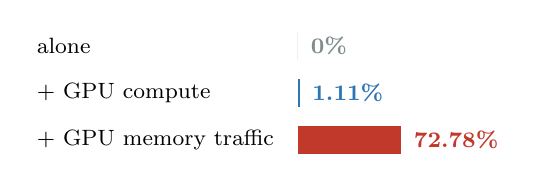
\begin{tikzpicture}[x=0.04cm, every node/.style={font=\footnotesize}]
  \foreach \y/\v/\c/\name in {0/0/gray2/alone, -0.6/1.11/accent/+ GPU compute, -1.2/72.78/red2/+ GPU memory traffic} {
    \node[anchor=west] at (0,\y) {\name};
    \fill[\c] (86,\y-0.18) rectangle ({86+\v*0.45},\y+0.18);
    \node[anchor=west, font=\footnotesize\bfseries, text=\c] at ({87+\v*0.45},\y) {\v\%};
  }
\end{tikzpicture}\\[0.3em]
{\scriptsize\color{gray2} camera deadline misses, Jetson Orin Nano} % CLAUDE
\end{columns}

\vspace{0.7cm}
\small
Where it varies: mostly outside the GPU, in the CPU, middleware and post-processing [5]. % CLAUDE (from preliminary-answers.md)
\\[0.3em]
Done so far: the experiment design for space and robot. % CLAUDE

\end{frame}

% ==================================================================
% 6. Next steps: written to read on its own
% Step 3 is Pulak's two questions from 5thNov-Updates.txt
\begin{frame}{Next steps}

\vspace{0.2cm}
\begin{enumerate}
  \setlength{\itemsep}{1.1em}
  \item \textbf{Measure.} Run a satellite VLM (Gemma 3 4B) and a robot VLA ($\pi_{0.5}$) on a Jetson Thor. Add other jobs, more load, lower precision and lower power one at a time, and count how often each request misses its deadline. % CLAUDE
  \item \textbf{Find where.} Split each late request into network, CPU wait and GPU run, to see which part made it late. % CLAUDE
  \item \textbf{Stabilise.} Try a CPU-GPU cooperative runtime or megakernel, and kernels rewritten in PTX/SASS, to make the latency more deterministic. % CLAUDE (from Pulak's two questions)
\end{enumerate}

\end{frame}

% ==================================================================
\begin{frame}{References}

\footnotesize
\begin{enumerate}
  \setlength{\itemsep}{0.5em}
  \item[{[1]}] J.\,M. Delfa Victoria, T.\,C. John, A.\,W. Herson. NAVI-Orbital: First In-Orbit Demonstration of a Zero-Shot Vision-Language Model for Autonomous Earth Observation. arXiv:2606.18271, 2026.
  \item[{[2]}] J. Tang, Y. Sun, et al. VLASH: Real-Time VLAs via Future-State-Aware Asynchronous Inference. arXiv:2512.01031.
  \item[{[3]}] Z. Yang, Q. Wang, et al. Jetson-PI: Towards Onboard Real-Time Robot Control via Foresight-Aligned Asynchronous Inference. arXiv:2607.12659, 2026.
  \item[{[4]}] T. Mei, C. Pei, et al. EdgePace: Deadline- and Freshness-Aware LLM Scheduling on Unified-Memory Platforms. arXiv:2610.37307, 2026.
  \item[{[5]}] L. Liu, Y. Wang, W. Shi. Understanding Time Variations of DNN Inference in Autonomous Driving. arXiv:2209.05487, 2022.
\end{enumerate}

\end{frame}

\end{document}
